%\documentclass[]{article}
\documentclass[]{standalone}
\usepackage{tikz}
\usepackage{amsmath}
\usetikzlibrary{arrows}
\begin{document}
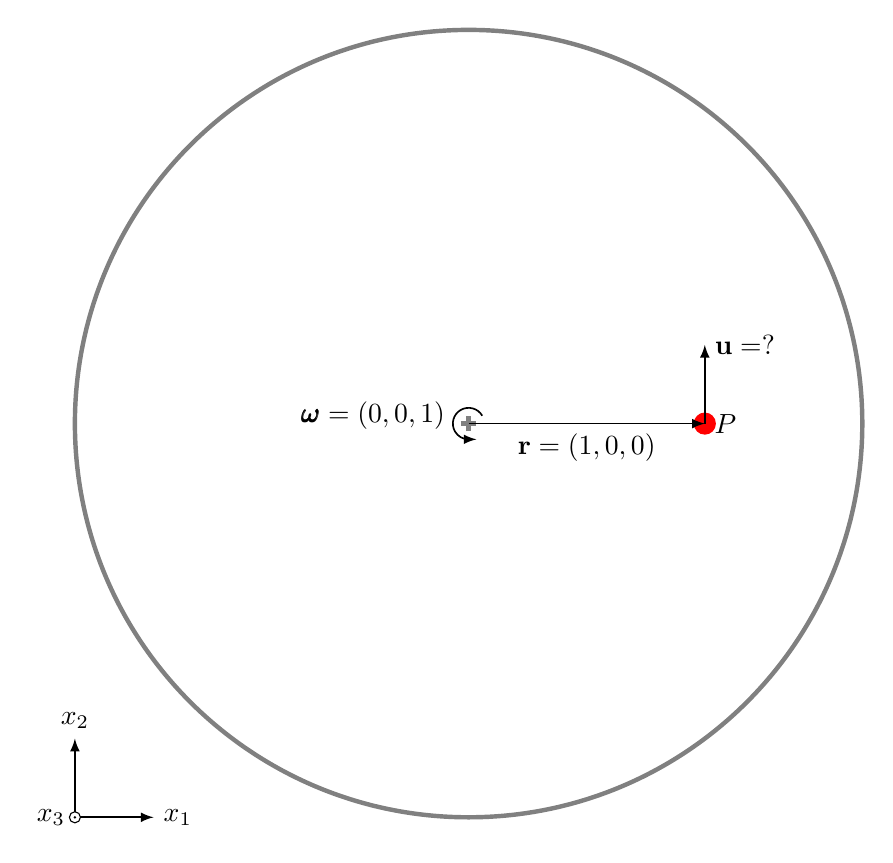
\begin{tikzpicture}
\draw [semithick, black,-latex] (-5,-5) -- (-4,-5) node[right]{$x_1$};
\draw [semithick, black,-latex] (-5,-5) -- (-5,-4) node[above]{$x_2$};
\draw [black, fill=white] (-5,-5) circle (2pt) node[below, left]{$x_3$};
\fill [black] (-5,-5) circle (0.5pt);
\draw [gray, ultra thick](0, 0) circle (5); % ...
\draw [gray, ultra thick](-0.1,0) -- (0.1,0); % ...
\draw [gray, ultra thick](0,-0.1) -- (0,0.1); % ...
\draw [semithick] (30:0.2cm) arc[radius=0.2, start angle=30, end angle=270] node[midway, left]{$\pmb\omega = (0,0,1)$};
\draw [semithick,-latex] (0,-0.2) -- (0.1,-0.2);
\fill [red] (3,0) circle (4pt) node[black, right]{$P$};
\draw [semithick, black,-latex] (3,0) -- (3,1) node[right]{$\mathbf{u}=?$};
\draw [semithick, black,-latex] (0,0) -- (3,0) node[midway, below]{$\mathbf{r}=(1,0,0)$};
\end{tikzpicture}
\end{document}

